A reach depth follows the flow through the reach, so like a lake stage it is a dependent variable that the Streamflow Routing (SFR) Package solves outside the groundwater flow matrix. The adjoint system is bordered in the same way as for a lake, described in Chapter~\ref{ch:lake}, with one equation per reach. What distinguishes the stream case is that those equations are not independent of one another: they carry the routing of water from reach to reach.

\section*{Reach equation}

\mf{} sets the depth $d$ of a reach so that the Manning discharge equals the mean of the flow entering and leaving it,

\begin{equation}
	\label{eqn:sfr-balance}
	q_{\mathrm{man}}(d) = \tfrac{1}{2}\left( Q_{\mathrm{in}} +
	Q_{\mathrm{out}} \right), \qquad
	Q_{\mathrm{out}} = Q_{\mathrm{in}} - Q_{\mathrm{leak}},
\end{equation}

\noindent where $Q_{\mathrm{leak}}$ is the exchange with the aquifer (L$^{3}$T$^{-1}$) and $d$ is the reach depth (L). For a reach without a cross section the wetted perimeter is the reach width, which carries no dependence on depth, so the discharge is a power of the depth,

\begin{equation}
	\label{eqn:sfr-manning}
	q_{\mathrm{man}}(d) = \frac{K w \sqrt{S}}{n}\, d^{5/3},
\end{equation}

\noindent with $w$ the width (L), $S$ the slope (dimensionless), $n$ Manning's roughness, and $K$ a unit conversion. The derivative needed for the border follows directly,

\begin{equation}
	\label{eqn:sfr-dqdd}
	\frac{\partial q_{\mathrm{man}}}{\partial d} = \frac{5}{3}
	\frac{q_{\mathrm{man}}}{d}.
\end{equation}

Equation~\ref{eqn:sfr-dqdd} is written in terms of the discharge \mf{} reports rather than rebuilding the rating from $K$, $w$, $S$, and $n$. The unit conversion in particular varies with the model's unit system, and taking the reported discharge makes the derivative correct without reproducing it.

Below a depth of $10^{-5}$ in model length units \mf{} smooths the discharge to zero. That smoothing is not reproduced, so a shallower reach is treated as carrying no flow.

\section*{Reaches with a cross section}

A reach may instead be given a cross section, a set of points describing the shape of the channel as a station across it and a height above the streambed. The channel is then a chain of straight segments between those points, and the discharge is the conveyance of the wetted part of each,

\begin{equation}
	\label{eqn:sfr-section}
	q_{\mathrm{man}}(d) = K \sqrt{S} \sum_{i} \frac{a_{i}^{5/3}}
	{n_{i} \, p_{i}^{2/3}},
\end{equation}

\noindent where $a_{i}$ is the wetted area of segment $i$ (L$^{2}$), $p_{i}$ is its wetted perimeter (L), and $n_{i}$ is Manning's roughness of the reach times the roughness fraction given for that segment. Equation~\ref{eqn:sfr-manning} is the special case of a single segment whose perimeter does not follow the depth, and equation~\ref{eqn:sfr-dqdd} does not hold for equation~\ref{eqn:sfr-section}.

Both the area and the perimeter of a segment follow the depth, so the derivative is taken from them rather than from a perturbation of the discharge,

\begin{equation}
	\label{eqn:sfr-dsection}
	\frac{\partial q_{\mathrm{man}}}{\partial d} = K \sqrt{S} \sum_{i}
	\frac{1}{n_{i}} \left(
	\frac{5}{3} \frac{a_{i}^{2/3}}{p_{i}^{2/3}}
	\frac{\partial a_{i}}{\partial d} -
	\frac{2}{3} \frac{a_{i}^{5/3}}{p_{i}^{5/3}}
	\frac{\partial p_{i}}{\partial d} \right).
\end{equation}

The area of a segment grows with the depth at its wetted top width, and its perimeter grows at the length of the wetted face, so both derivatives in equation~\ref{eqn:sfr-dsection} come from the geometry of the section and neither needs the discharge. Both step where the water surface passes a point of the section, and the derivative is taken on the side the depth is on.

A cross section carries a second consequence. The streambed conductance of a reach is proportional to its wetted perimeter, and for a section that perimeter follows the depth, so the leakage responds to the depth through the conductance as well as through the stage,

\begin{equation}
	\label{eqn:sfr-dleak}
	\frac{\partial Q_{\mathrm{leak}}}{\partial d} = C \left(
	1 + \frac{1}{P} \frac{\partial P}{\partial d}
	\left( h_{s} - h \right) \right),
\end{equation}

\noindent where $C$ is the streambed conductance (L$^{2}$T$^{-1}$), $P$ is the wetted perimeter of the whole section (L), $h_{s}$ is the reach stage (L), and $h$ is the head beneath the reach (L), taken at the bottom of the streambed where the reach is perched. A reach without a cross section has a perimeter that does not follow the depth, the bracket in equation~\ref{eqn:sfr-dleak} is one, and the leakage derivative is the conductance alone. Only the bracket is formed from the section, so the conductance the package reports sets the magnitude and a reach on an inactive cell stays at zero.

\section*{Routing}

The flow entering a reach is the sum of the flows leaving the reaches upstream of it, apportioned by the diversion fractions specified for the network. The connectivity is that of the stream network itself, which identifies the reaches upstream of each reach.

Because $Q_{\mathrm{out}}$ of an upstream reach depends on that reach's depth and on its leakage, differentiating equation~\ref{eqn:sfr-balance} produces entries away from the diagonal in two places. The first couples one reach row to another,

\begin{equation}
	\label{eqn:sfr-updepth}
	\frac{\partial}{\partial d_{u}} \; \tfrac{1}{2} Q_{\mathrm{in}} =
	\tfrac{1}{2}\, \sigma \, \frac{\partial q_{\mathrm{man},u}}
	{\partial d_{u}},
\end{equation}

\noindent where $\sigma$ is the fraction of the upstream reach's outflow routed to this one (dimensionless). The second reaches back into the aquifer, because the flow leaving the upstream reach carries half of that reach's leakage,

\begin{equation}
	\label{eqn:sfr-uphead}
	\frac{\partial}{\partial h_{u}} \; \tfrac{1}{2} Q_{\mathrm{in}} =
	\tfrac{1}{2}\, \sigma \, \mathrm{HCOF}_{u}.
\end{equation}

The sign of equation~\ref{eqn:sfr-uphead} is easy to get wrong, and an error there is not obvious in the result: it produces sensitivities of a plausible magnitude that are wrong by a modest factor. Checking the assembled block against a finite-difference Jacobian is what identified it.

\section*{Flow-limited reaches}

A reach can be asked to lose more water than it carries. \mf{} limits the leakage to the available flow, and marks that state by leaving both the reach's \texttt{HCOF} and the change in its outflow at zero: the reach passes on nothing and its leakage no longer responds to the head beneath it.

The derivative structure changes accordingly. The reach's own depth no longer sets its leakage, so the coupling moves to the reaches upstream that supply it, and a correction appears that connects one aquifer cell directly to another, bypassing the reach equation. That correction is folded into the aquifer block of the bordered matrix rather than the border itself.

\section*{Verification}

\begin{figure}[htb]
	\centering
	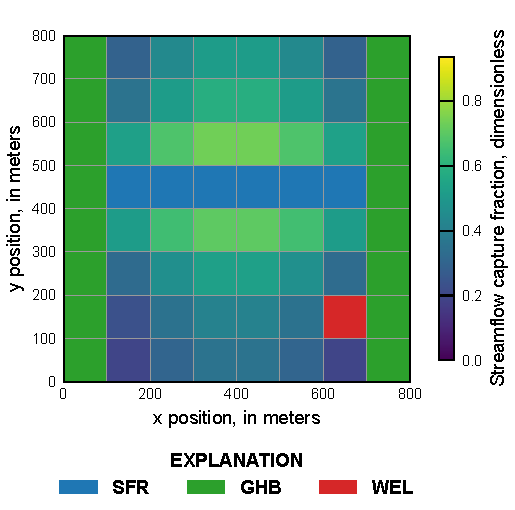
\includegraphics{Figures/sfr-capture.pdf}
	\caption{Streamflow capture fraction for the model the streamflow tests
	use, the fraction of a withdrawal at a cell that is drawn from the stream
	rather than from storage or from another boundary. SFR marks the cells the
	reaches occupy, GHB the general-head boundaries that hold the heads at the
	left and right edges of the model, and WEL the pumped cell. The reach depths
	are solved with the flow equations as described in this chapter.}
	\label{fig:sfr-capture}
\end{figure}

A chain of reaches crossing a single layer model was pumped from a cell away from the stream, and the resulting change in reach exchange compared with the difference between two forward runs. The adjoint reports a capture of $-2.32472 \times 10^{-1}$ against a two-run difference of $-2.32470 \times 10^{-1}$. Capture fractions across that model are shown in figure~\ref{fig:sfr-capture}. On a valley model routing a longer network, holding the reach depths fixed gave a discrepancy of about 26 percent, and solving the reach equations with the flow equations reduced it to 0.04 percent.

A branching network, in which one reach receives water from two upstream reaches and the apportionment fractions therefore matter, reproduces its finite-difference sensitivities to the same tolerance.

A diversion was added to the same model and run under each of the four rules. Holding the diverted flow fixed gave sensitivities in error by 0.03 to 0.11 percent under the three rules whose derivative is not zero, and carrying equations~\ref{eqn:sfr-passed} and \ref{eqn:sfr-diverted} brought all four to within 0.001 percent. Under \texttt{THRESHOLD} the derivative is zero, and holding the flow fixed was already exact.

The same model was run again with a trapezoidal cross section on every reach. The rating of equation~\ref{eqn:sfr-section} reproduces the discharge the forward model solved each depth against to eleven significant figures, which is the check that established the geometry before any derivative was taken from it, and the derivative of equation~\ref{eqn:sfr-dsection} matches a central difference of that rating to nine, on both sides of a break in the section. Holding the depths of those reaches fixed gave a capture sensitivity in error by 1.7 percent, and carrying equations~\ref{eqn:sfr-dsection} and \ref{eqn:sfr-dleak} reduced it to 0.002 percent.

\section*{Diversions}

A diversion takes water out of the flow a reach passes on, under one of four rules. Writing $v$ for the rate the diversion is given (L$^{3}$T$^{-1}$, or dimensionless for a fraction) and $q$ for the flow available to it when its turn comes (L$^{3}$T$^{-1}$), the rules and the derivative each carries are given in Table~\ref{tab:sfr-rules}.

\begin{table}[htb]
	\centering
	\caption{The four diversion rules, the flow each takes, and how that flow
	follows the flow available to the diversion.}
	\label{tab:sfr-rules}
	\small
	\begin{tabular}{lll}
		\toprule
		Rule & Diverted & $\partial / \partial q$ \\
		\midrule
		\texttt{FRACTION}  & $q v$          & $v$ \\
		\texttt{EXCESS}    & $\max(q - v, 0)$ & 1 above $v$ \\
		\texttt{UPTO}      & $\min(v, q)$     & 1 below $v$ \\
		\texttt{THRESHOLD} & $v$ if $q \geq v$ & 0 \\
		\bottomrule
	\end{tabular}
\end{table}

Three of the four are piecewise, so the derivative steps where the rule switches, in the same way that the derivative of a lake connection steps as the connection becomes perched. That is workable away from the switch.

Which rule is in effect cannot be read from the simulation, because \mf{} keeps it as text rather than among the quantities it exposes. It does not have to be. The flow available to a diversion, the rate it was given, and the flow it took are all recoverable, and those three determine the derivative. Where two rules give the same diverted flow they also give the same derivative: \texttt{THRESHOLD} and \texttt{UPTO} both hold at the rate once the flow exceeds it, and \texttt{THRESHOLD} and \texttt{EXCESS} both take nothing below it. The rule itself can therefore stay unknown.

The diversions of a reach are applied in turn, each taking from what the one before it left, so writing $g_{i}$ for the derivative of diversion $i$ the flow passed on to the reaches below carries

\begin{equation}
	\label{eqn:sfr-passed}
	\frac{\partial q_{\mathrm{out}}}{\partial q} = \prod_{i} \left( 1 - g_{i} \right),
\end{equation}

\noindent and the reach a diversion feeds receives

\begin{equation}
	\label{eqn:sfr-diverted}
	\frac{\partial q_{i}}{\partial q} = g_{i} \prod_{j < i} \left( 1 - g_{j} \right).
\end{equation}

Equations~\ref{eqn:sfr-passed} and \ref{eqn:sfr-diverted} scale the routing coefficient of equation~\ref{eqn:sfr-updepth} rather than adding structure of their own, so a diversion enters the bordered system only through the share one reach sends another. The share itself is taken from the total \mf{} keeps for each reach, which leaves out both a diversion and an inactive reach, rather than summed from the fractions given to the reaches below, which would count a diversion in the denominator.

\section*{Limitations}

The flows leave the rule open only where two rules divert the same amount and respond differently, which takes a coincidence between the flow available and the rate the diversion is given. A flow of exactly twice the rate is one: \texttt{EXCESS} passes the rate on and takes the rest, which is then the rate itself, the same amount \texttt{UPTO} and \texttt{THRESHOLD} take, and the three do not agree on how that amount would change. Where that happens \adj{} reports the diversion and holds its flow fixed rather than returning a partial derivative silently.

A reach whose outflow is not positive diverts nothing under any rule, and passes nothing on, so no rule is inferred for it and none is needed.
